\documentclass[12pt,a4paper, oneside]{scrartcl}
\usepackage[utf8]{inputenc}
\usepackage[ngerman]{babel}	%language
\usepackage{hyperref}	% to link mail adress
\usepackage{graphicx}	% to link images in document
\usepackage{xcolor}		% Für die Farben der Überschriften, wenn das überhaupt funktioniert
\usepackage[numberedbib]{apacite}	% Zum Zitieren nach dem APA Standard


% leichtes / helles Blau für die Überschriften
\definecolor{light blue}{RGB}{0 170 255}

% neue Commands
\newcommand*{\quelle}[1]{\par\footnotesize Quelle:~#1}

% Titel des Dokumentes
\title{\small{Universität Trier \\ Fachbereich 4 \\ Informatik}}
\date{}

\begin{document}
%------------------------------------------ Titel -----------------------------------------
\maketitle

\begin{center}
	% größerer Abstand zwischen Bild und Text
	\vspace{0.5cm}
	
\includegraphics[width=0.7\textwidth]{Logo_Universitaet_Trier} \\
	\vspace{1cm}
	
	% Titel
	Exposé für das Praktikum im großen Studienprojekt mit dem Thema: 
	\textbf{(Collaborative) Mobile-AR Sculpting}
\end{center}
%------------------------------------------------------------------------------------------
\vspace{2cm}

%------------------------------------------ Autoren -----------------------------------------
\begin{flushleft}
	von: \\
	\vspace{0.5cm}
	Sebastian Britner \\
	\href{mailto:s4sebrit@uni-trier.de}{s4sebrit@uni-trier.de} \\
	Matrikelnummer: 1485271 \\
	Fachsemester: 04 \\
	\vspace{0.5cm}
	Jan Niclas Ruppenthal \\
	\href{mailto:s4jsrupp@uni-trier.de}{s4jsrupp@uni-trier.de} \\
	Matrikelnummer: 1481198 \\
	Fachsemester: 04 \\
\end{flushleft}
%------------------------------------------------------------------------------------------


\newpage


%------------------------------------------ Inhaltsverzeichnis ------------------------------------
\tableofcontents

%------------------------------------------------------------------------------------------


\newpage


%------------------------------------------- Einleitung -----------------------------------
\section{Einleitung}

Augmented Reality (AR) ist als digitale Erweiterung der Realität schon in einigen Branchen im Einsatz. Ob in der Unterhaltung, der Industrie, dem Einzelhandel oder der Bildung, AR findet zahlreiche Anwendungsgebiete \cite{conrad}. 
Auch wenn nach den anfänglichen Erfolgen im Jahr 2016 das Wachstum der AR Branche nach Marktanalyse einer Extended Reality Studie im Jahr 2020 doch moderater ausfiel als prognostiziert, bleibt das Potenzial dieser innovativen Technologie groß \cite{marktanalyse_AR}.
Ein besonders interessanter Bereich ergibt sich bei der Entwicklung von Mobile AR Applikationen. Mobile Augmented Reality (MAR) beschreibt dabei AR, die man überall mit hinnehmen kann und auf üblichen mobilen Geräten wie Smartphones oder Tablets nutzen kann \cite{craig_2013}.
Damit können AR Applikationen zu jeder Zeit und an jedem Ort erfahren werden, wodurch dem Nutzer eine einfache und angenehme Möglichkeit geboten wird AR überall in der realen Welt zu verwenden.

	
	
%------------------------------------------- Motivation -----------------------------------
\subsection{Motivation}
	
Heutzutage wird MAR in diversen Applikationen wie zum Beispiel „Snapchat" \cite{snapchat} und „Pokémon GO" \cite{pokemon_go} genutzt. 
Wie Konsumentenbefragungen ergeben, sind ein Großteil der Menschen und besonders jüngere Generationen schon einmal in Kontakt mit solchen AR Applikationen gekommen \cite{umfrage_2016}. Besonders „Pokemon GO“ konnte innerhalb kürzester Zeit Millionen neuer Nutzer und Nutzerinnen begeistern \cite{tobien_2016}.
Auch wenn die angeführten Applikationen eher dem Bereich der Unterhaltung zuzuordnen sind, finden wir dennoch, dass AR auch außerhalb der Unterhaltungsbranche großes Potenzial besitzt. Denn mit MAR wird eine neue wahrnehmbare Dimension geschaffen, der es lediglich mobilen Geräten zur Wahrnehmung bedarf. Mit AR sind wir in der Lage mit einen beliebigen Raum zu interagieren. Dabei wird mit Hilfe eines Tiefeneindrucks durch die eigentlichen zweidimensionalen Abbildungen ein räumlicher Eindruck vermittelt. 
Weiterhin spielt hierbei die räumliche Registration, also die Herstellung des dreidimensionalen Bezugs der virtuellen Objekte zum realen Raum eine entscheidende Rolle zur Aufrechterhaltung der Illusion. Dabei passt sich das virtuelle Objekt in Abhängigkeit der Position des Beobachters räumlich an, sodass es nicht als willkürlich, sondern als in den Raum integriert wahrgenommen wird \cite{trinler_2009}.
Damit kann man sich also jeden beliebigen Ort aneignen und ihn damit als  Umgebung für die Darstellung von virtuellen Objekten verwenden. Gleichzeitig kann dieser Raum durch die Bereitstellung unterschiedlichster Interaktionsmöglichkeiten erfahren werden. 
Die neue Dimension erlaubt es auf dem Bestehenden und Vorhergehenden aufzubauen und für eine neue Verbundenheit mit Orten zu sorgen.
Überall, wo Umgebung wahrgenommen werden kann, kann AR unsere Wahrnehmung unterstützen oder beeinflussen.
Mithilfe von AR kann die Außenwelt in ihrer Fülle miteinbezogen werden.
So können Nutzer beispielsweise die Größe von Objekten in Bezug auf die Realität besser einschätzen. Außerdem können sich die Objekte jeden beliebigen Raum aneignen, damit man das erschaffene virtuelle Objekt in Bezug auf den Raum besser wahrnehmen kann. 
Ein weiteres Gebiet, welches sich diese Eigenschaft zunutze machen kann und damit auch durch dieses Projekt bedient werden könnte, ist Produktdesign. Damit wird durch die Integration von AR Technologien in die Produktentwicklung die Fehlererkennung in den frühen Phasen des Designs und damit das Vertrauen der Teilnehmer in ihr Design erhöht. \cite{mourtzis_2018}.
Zusätzlich könnte mit diesem Projekt die künstliche Ausdrucksform und die Kreativität bei konstruktiver Kunst unterstützt werden. So stellte eine Gruppe im bekanntesten und ältesten Museum in New York AR Kunstwerke auf \cite{urbanshit_2018}. Die Besucher des Museums mussten nur ihre Smartphones auf die Werke in der Sammlung richten, um die virtuelle Kunst wahrnehmen zu können (siehe \autoref{figure_MoMAR}). \\
\begin{figure}[h!]
\centering
\includegraphics[scale=0.3]{MOMAR_Bild}
\quelle{\cite{ehrenkranz_2018}}
\caption{Digitales Kunstwerk in MoMA, New York}
\label{figure_MoMAR}
\end{figure} \\
Auch der Vorteil von digitalen Museen spielt hier eine wichtige Rolle. Die Besucher eines digitalen Museums gewinnen nähere Erfahrungen auch mit weitentlegener Kunst, da sie bereits von anderen erstellte Skulpturen in ihre Umgebung projizieren und wahrnehmen können. Des Weiteren werden viele junge Besucher durch die Vereinigung konservativer Kunst mit neuer Technologie angesprochen und es werden zusätzlich Lerneffekte mit Unterhaltung vereint.


%-------------------------------------------------------------------------------------------------------

	
\newpage

	
%------------------------------------------- Problemstellung -----------------------------------	
	
\subsection{Problemstellung}

Aufgrund des technischen Fortschritts im IT-Sektor erweitern sich auch die Anwendungsfelder \cite{gal_digital_gmbh_2019}. So ergibt sich auch im Bereich der konstruktiven Kunst ein interessantes Themenfeld.
Die einfache Projektion von Elementen in die reale Umgebung lässt sich durch die Implementierung von Gestaltungsmöglichkeiten erweitern, wodurch sich eine neue Verbindung des/der Nutzers/Nutzerin zur erweiterten Realität herstellen lässt, die dem/der Nutzer*in durch die eigenständigen Einflussmöglichkeiten mehr Kreativität ermöglichen soll. Dieser Einfluss soll darin bestehen Objekte zu Skulpturen zusammensetzen zu können. Dabei soll dem/der Nutzer*in die Möglichkeit gegeben werden diese virtuellen Kunstwerken aus auswählbaren virtuellen Materialien in einem realen physischen Raum zu errichten. Hierzu werden ihm/ihr Tools bereitgestellt, die das Auswählen, Rotieren, Verändern, sowie das Verbinden von Formen ermöglichen sollen. Hürden ergeben sich dabei vor allem in der reibungslosen Gestaltung der Nutzerinteraktion. Die Problematik besteht zum einen darin, welche Interaktionsmethode gewählt wird, um dem/der Nutzer*in die Auswahl und die Manipulation von Formen zu ermöglichen. Zum anderen sehen wir auch die Größe des Displays als weitere Problematik bei der Anordnung der Elemente der UI.
Dabei soll es dem/der Nutzer*in möglichst einfach und verständlich gemacht werden mit der Umgebung und den virtuellen Formen zu interagieren, um damit auch die Illusion der Verbundenheit der Realität und der Virtualität aufrecht zu erhalten.


%-------------------------------------------------------------------------------------------------------



\newpage



%----------------------------------------------Verwandte Arbeiten--------------------------------------

\section{Verwandte Arbeiten}
In diesem Abschnitt werden Arbeiten zur vorgestellten Domäne besprochen, die sich mit der Gestaltung angemessener AR Schnittstellen, sowie der Verwendung entsprechender Techniken auseinandergesetzt haben.
Eine Reihe von Arbeiten ergeben sich aus dem 2017 ausgetragenen IEEE 3DUI Contest \cite{guo_mcmahan_weyers_2017}. Dieser stellt die Rahmenbedingungen wie die Gestaltung der AR Applikation für Smartphones ohne die Nutzung weiterer Geräte oder Sensoren vorauszusetzen und dabei besonders auf die für die optimale Nutzerinteraktion notwendigen sechs Freiheitsgrade  (6DOF) zu achten. Dabei wird zwischen den Freiheitsgraden für das Positionieren und für die Rotation unterschieden \cite{guo_mcmahan_weyers_2017}. \\
Für die Gestaltung der in unserem Projekt vorgesehenen Interaktionstechnik lohnt sich zunächst ein Blick in die bekannten Umsetzungen aus anderen Projekten.
Das Interaktionsmodell HOT nutzt dabei bedruckte Karten, die zur Bereitstellung bestimmter Funktionen in das Kamerasichtfeld gebracht werden können \cite{attanasio_2017}. 
Durch die Verwendung von Karten in HOT ergibt sich eine Entlastung der auf dem Bildschirm bereitzustellenden Tools zur Bearbeitung der Formen und somit eine Entdigitalisierung der Sicht, die den Eindruck der Koexistenz zwischen Realität und Virtualität erhöht.
In unserem Projekt implementieren wir die Karten nicht zur Manipulation, sondern als Feature zur Bereitstellung von Skulpturexemplaren, da wir die Vorzüge von Karten nutzen wollen, aber gleichzeitig dafür sorgen wollen, dass die Verwendung der Applikation weniger Abhängigkeit von Hilfsmitteln besitzt. Dadurch soll gewährleistet werden, dass die Applikation auch spontan angewendet werden kann. \\
Zur Umsetzung der Steuerung in HOT wird dabei eine Manipulationstechnik angewandt, die auf dem Konzept von Direktheit und Unabhängigkeit basiert. Dabei können Objekte bewegt oder skaliert werden, ohne das zu manipulierende Objekt direkt zu berühren.
Weiterhin sieht diese Technik die vollständige Manipulation von Objekten in 6 Freiheitsgraden über die Verwendung von lediglich zwei mit dem Bildschirm in Kontakt stehenden Fingern vor. Hierbei werden zwei Modi und zwei entsprechende Gesten eingeführt, wobei die Bewegungsmuster der beiden Finger für die Auswahl des entsprechenden Modus entscheidend sind \cite{liu_2012}. Dadurch hat der Nutzer größere Freiheiten bei der Steuerung und es ergibt sich eine angenehmere Verwendung des Geräts auf dem die AR Applikation läuft. Aus diesem Grund verwenden wir das Konzept der Fingerbewegung in unserem Interaktionsmodell zur Änderung der Größe und der Form. \\
Bei dem Interaktionskonzept T4T durchläuft die Interaktion drei Phasen, die als marker-tracking, cursor mode und tuning mode bezeichnet werden \cite{cannavo_2020}.
In der ersten Phase muss der Nutzer die Markierung mit der Kamera des Mobilen Geräts erfassen. Anschließend wechselt das System automatisch in den cursor mode, bei dem ein Cursor genutzt wird, dessen Position und Bewegung an die Ansicht des Gerätes gebunden ist, um Objekte auszuwählen. Wird der Cursor für eine kurze Zeit auf ein Objekt gerichtet, so wird das Objekt ausgewählt und man gelangt in den tuning mode. In diesem Modus wird ein Pop-Up Menü geöffnet, welches verschiedene Funktionalitäten zur Manipulation des Objekts bereitstellt \cite{cannavo_2017}. Damit werden die verfügbaren Optionen an die aktuelle Situation angepasst, was uns auch dazu bewegt hat die Interaktion in zwei Phasen zu unterteilen. 
Darüberhinaus wird im Interaktionsmodell T4T zur Manipulation des Objektes ein Drehknopf als UI-Element verwendet, der eine feinere Änderung der Parameter vorsieht. Da bestimmte Parameter wie die Rotation entlang der Achsen präziser geschehen muss, verwenden wir ebenfalls UI-Elemente für diese Art der Manipulation. \\
Aufgrund des kleinen Displays und der Batterie benötigt man andere Interaktionstechniken als mit einem Head-mounted Display. Dazu gibt es drei grundlegende Techniken zur Interaktion mit MAR \cite{goh_sunar_ismail_2019}: 
\begin{itemize}
\item \textbf{touchbasiert:} \\
Hierbei werden die Finger benutzt, um 3D Objekte zu manipulieren, wobei die Rotation das größte Problem ist. 
\item \textbf{mid-air gestenbasiert:} \\
Mithilfe von Gestenerkennung werden Gesten erkannt, die vorher als bestimmte 3D Objekt Manipulationen definiert wurden. 
\item \textbf{gerätebasiert:} \\
Diese Technik benötigt die Attribute des Geräts, wie zum Beispiel Position und Winkel. Dabei dient das Gerät als ein Controller für den Benutzer. 
\end{itemize}
Die Vorteile der gerätebasierten Interaktion nutzen wir in unserem Projekt für die Manipulation der Position des Objekts. Durch alle drei Interaktionstechniken können Nutzer die Formen in sechs Freiheitsgraden (6DOF) manipulieren. Jedoch ist die größte Schwierigkeit bei allen Interaktionstechniken die Verdeckung durch die Finger \cite{goh_sunar_ismail_2019}. \\
%Ebenfalls essenziell sind die Auswirkungen der Distanz zwischen den virtuellen Objekten und dem Nutzer. In einem Experiment konnten Probanden mithilfe der Stimme, mehreren Gesten oder mit einer Fernbedienung (die Wii Remote) in einer Entfernung von 8, 12 und 16 Fuß mit den virtuellen Objekten interagieren. Die Probanden hatten als Aufgabe die virtuellen Objekte zu selektieren, zu rotieren und zu verschieben. Dabei erzielten die Interaktionen mithilfe der Wii Remote die besten Ergebnisse bei allen drei Aufgaben. Auch die gestenbasierte Interaktionen schnitt bei den letzten beiden Aufgaben gut ab 
%In einer Umfrage der Probanden wurde festgestellt, dass gestenbasierte Interaktionen am einfachsten und die stimmbasierten Interaktionen am schwersten zu benutzen waren
%\cite{whitlock_harnner_brubaker_kane_szafir_2018}. \\
In einer weiteren Forschungsarbeit wurden die Möglichkeiten der kollaborativen AR in durchgeführten Experimenten gezeigt. Ein positiver Aspekt der MAR ist die spontane Kollaboration zwischen Nutzer in Bezug auf die Manipulation komplexer 3D Modelle. Der große Nachteil von CSCW Desktop Applikationen ist, dass die Benutzer untereinander und von ihren Werkzeugen getrennt werden. AR beseitigt diese Nachteile, da die Werkzeuge der Nutzer in der wirklichen Umgebung eingebettet werden können. Zudem können mit AR persönliche Arbeitsbereiche erschaffen werden und die Benutzer interagieren mit den vorhandenen Funktionen auf einer natürlichen Weise \cite{reitmayr_schmalstieg}. \\
\\
Aus der Betrachtung ergibt sich, dass die verschiedenen Interaktiontechniken unterschiedliche Vor- und Nachteile zur Manipulation bestimmter Parameter nach sich ziehen. Wir vereinen bestimmte Elemente der Interaktionsmodelle, um ein Konzept zu erstellen, was parameterspezifisch die entsprechenden Interaktiontechniken anwendet. 
Auch die angesprochene Strukturierung der Interaktion in Phasen wenden wir in unserem Konzept an.
Wir konzentrieren uns bei der Umsetzung auf die optimale Interaktion eines Nutzers und versuchen davon ausgehend die Grundlage zu schaffen für eine kollaborative Manipulationstechnik, auf die wir in diesem Projekt aber nicht näher eingehen.



%-------------------------------------------------------------------------------------------------------



\newpage



%----------------------------------------------Projektzielsetzung--------------------------------------

\section{Projektzielsetzung}
Das Ziel des Projekts ist es mit Hilfe von Unity und Vuforia ein benutzerfreundliches AR-Interface zu gestalten, so wie dem Nutzer alle Funktionen zur Manipulation von Formen und damit zum Bau von Skulpturen bereitzustellen.
Dafür lässt sich die Interaktion wie beim Interaktionskonzept T4T am besten in mehrere Phasen unterteilen. Dabei haben wir uns für einen Auswahlmodus und einen Manipulationsmodus entschieden. Der Auswahlmodus dient dazu virtuelle Objekte zu markieren oder zu platzieren. Hierbei sollen dem Nutzer mehrere verschiedene Objekte in einer scrollbaren Seitenleiste zur Auswahl bereit gestellt werden. Um Objekte zu platzieren, verwenden wir einen transparenten, zentrierten Cursor, der auf die Position im Raum zeigt, wo das Objekt platziert werden soll. Im Gegensatz zu T4T wird unser Cursor nicht zur Markierung von Formen genutzt, sondern dies geschieht über das Antippen des Objektes auf dessen Darstellung. Diese Selektion nennt man auch screen-based selection. (siehe \autoref{figure_GUI_A}).
\begin{figure}[h!]
\centering
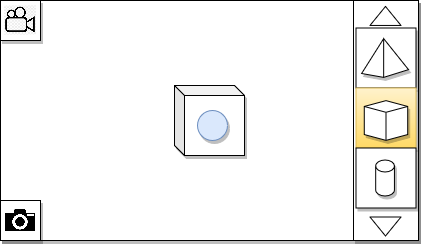
\includegraphics[scale=0.4]{GUIAuswahlmodus}
\caption{Die GUI im Auswahlmodus}
\label{figure_GUI_A}
\end{figure}
%
\\
%
Wurde eine Form markiert, gelangt der Nutzer in den Manipulationsmodus, wo ihm/ihr verschiedene Funktionen zur Bearbeitung der Form zur Verfügung gestellt werden. In \autoref{figure_M} sind die Manipulationsmethoden sowie in \autoref{figure_GUI_M} deren Darstellung in der GUI im Manipulationsmodus abgebildet.
\begin{figure}[ht!]
\centering
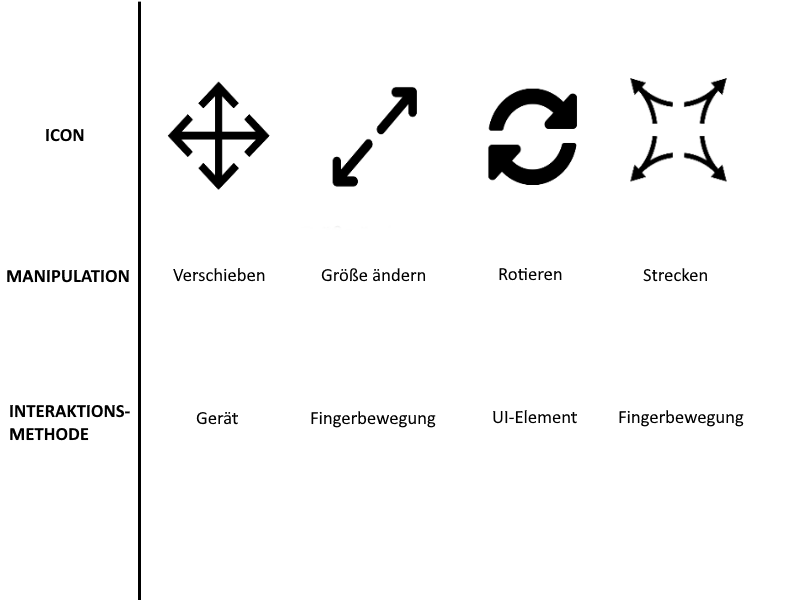
\includegraphics[scale=0.375]{Manipulationsmethoden}
\caption{Die verschiedenen Manipulationsmethoden}
\label{figure_M}
\end{figure}
%
\\
%
\\
\begin{figure}[ht!]
\centering
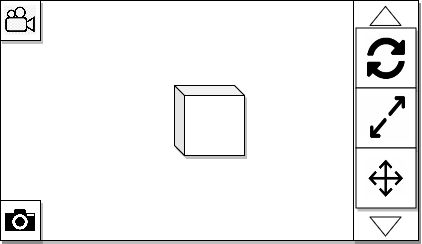
\includegraphics[scale=0.4]{GUIManipulationsmodus}
\caption{Die GUI im Manipulationsmodus}
\label{figure_GUI_M}
\end{figure}
\\
Wie zuvor beschrieben haben wir den verschiedenen Arten von Manipulationen bestimmte Interaktionstechniken zugewiesen. So erfolgt die Verschiebung eines Objekts über das Gerät, die Veränderung der Größe und der Form über Fingerbewegungen und die Rotation mit Hilfe eines UI-Elements. \\
Weiterhin sollen verschiedene Features für eine bessere Nutzererfahrung sorgen. Zu diesen zählen zum einen das Festhalten von besonderen Momenten durch die Screenshot- und Aufnahmefunktion (siehe \autoref{figure_GUI_A} und \autoref{figure_GUI_M}). 
Zum anderen sollen wie beim Interaktionsmodell HOT Karten verwendet werden, die jedoch keine Funktion bereit stellen, sondern als Veranschaulichung von Beispielen fungieren sollen. Dabei soll das Modell bei näherer Betrachtung in seine Einzelteile aufgespalten werden, sodass man die Zusammensetzung aus den einzelnen Teilen erkennen kann \cite{youtube_unity}. Durch dieses Feature benötigt der/die Nutzer*in keine Anleitung zum Aufbau bestimmter Skulpturen. Gleichzeitig kann Platz auf dem Display eingespart werden und ein unmittelbarer Nachbau der Skulptur erfolgen.\\

%-------------------------------------------------------------------------------------------------------



\newpage



%----------------------------------------------Arbeitsplan--------------------------------------

\section{Arbeitsplan}
\textbf{Dauer}: 18 Wochen (05.05.2021 - 09.09.2021) \\
%
\\
\begin{tabular}{|l|c|c|}
\hline
Datum & Arbeitspaket & Zugewiesen an \\
\hline
Bis 12.05. & Recherche zu Unity AR und Vuforia & Beide \\
\hline
Bis 15.05. & GUI Paperprototyp \& Test & Beide \\
\hline
Bis 01.06. & Unity: GUI im Auswahlmodus  & Beide \\
\hline
Bis 13.06. & Unity: GUI im Manipulationsmodus & Sebastian \\
\hline
Bis 01.08. & Funktionen zur GUI im Auswahlmodus & Jan Niclas \\
\hline
Bis 01.08. & Funktionen zur GUI im Manipulationsmodus & Sebastian \\
\hline
Bis 07.08. & Test \& Bugfixing & Beide \\
\hline
Bis 01.09. & 3D Modelling für die Beispiele + Animationen & Jan Niclas \\
\hline
Bis 09.09. & Test \& Bugfixing der Features & Beide \\
\hline
Bis 09.09. & Präsentation vorbereiten & Beide \\
\hline
Am  09.09. & Abgabe des Projekts & \\
\hline
Am  16.09. & Präsentation des Projekts & \\
\hline
\end{tabular}

%-------------------------------------------------------------------------------------------------------


\newpage



%---------------------------------------------->Literaturverzeichnis--------------------------------------
\bibliographystyle{apacite}
\bibliography{bibliography.bib}
%-------------------------------------------------------------------------------------------------------


\end{document}
